%!TEX root = ../../dokumentation.tex

\section{Application-Layer}
Die vierte Schicht des \ac{IoT}-Application Stack ist das Application Layer. Im Application Layer geht es darum, die vernetzten Geräte für den Nutzer verwendbar zu machen. Hierfür werden Applikationen entwickelt. Im Falle des \ac{IoT} Smart-Locks sollte dies eine Handy-Applikation sein, welche die Kommunikation des Nutzers mit dem Schloss ermöglicht.

Die Anforderungen an die App sind recht simpel: Der Nutzer soll die Schlösser in der App angezeigt bekommen und nahegelegene Schlösser entsperren können. Die Anzeige soll zweiermaßen ermöglicht werden. Einerseits soll eine simple Liste die Schlösser aufführen. Zusätzlich soll auch eine Karte die Geo-Positionen der Schlösser mit hoher Genauigkeit anzeigen, um speziell dem Verlustpotential entgegenzuwirken. Der Nutzer soll nahegelegene Schlösser entsperren können. Der Zusatz nahegelegen ist hierbei wichtig, da die Ver- bzw. Entriegelung des Schlosses aus großer Distanz möglich sein soll.

Die App setzt genau obige Anforderungen um. Mithilfe einer Navigation Bar kann zwischen der Listen- und der Kartenansicht gewechselt werden. Nahegelegene Schlösser können Ver- und Entriegelt werden. Dem Benutzer werden alle Schlösser sowohl in der Such-Liste, als auch auf der Karte angezeigt (Abbildung \ref{fig:search}, \ref{fig:map}).

Die Kommunikation der App läuft zweigeteilt: Zum einen empfängt die App die Geo-Positionen der Schlösser über \ac{HTTP} von dem Node-Red Server. Zum anderen kann über die \ac{BLE}-Konnektivität des Smartphones mit nahegelegenen Schlössern kommuniziert werden (Abbildung \ref{fig:connected}).

\begin{figure}[!htbp]
    \centering
    \subfloat[Karte mit markierter Position]{
        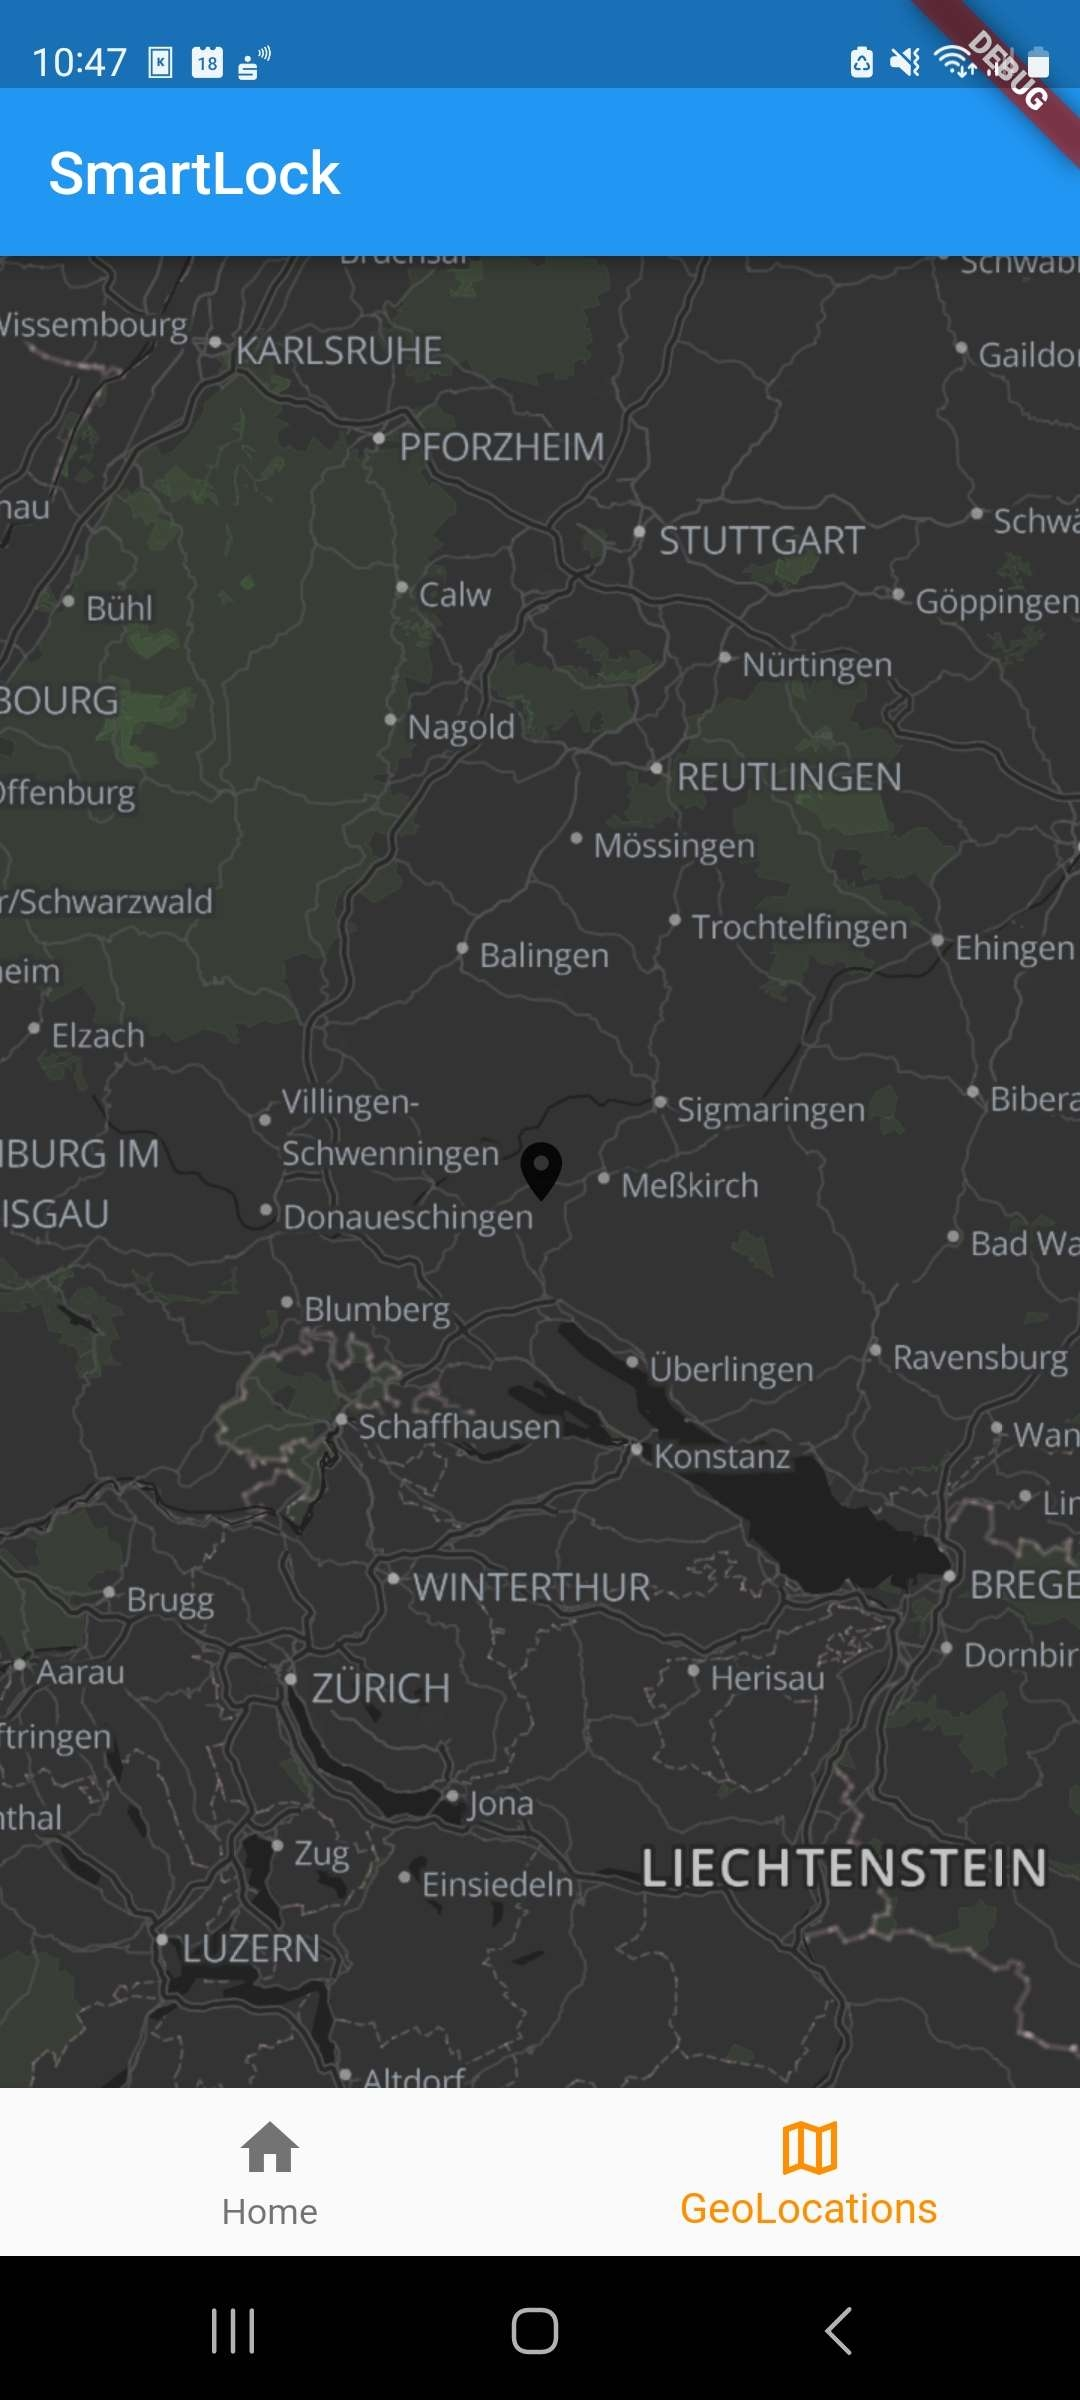
\includegraphics[width=0.3\textwidth]{images/map.jpg}
        \label{fig:map}
    }
    \hfill
    \subfloat[Suche nach Schloss über BLE]{
        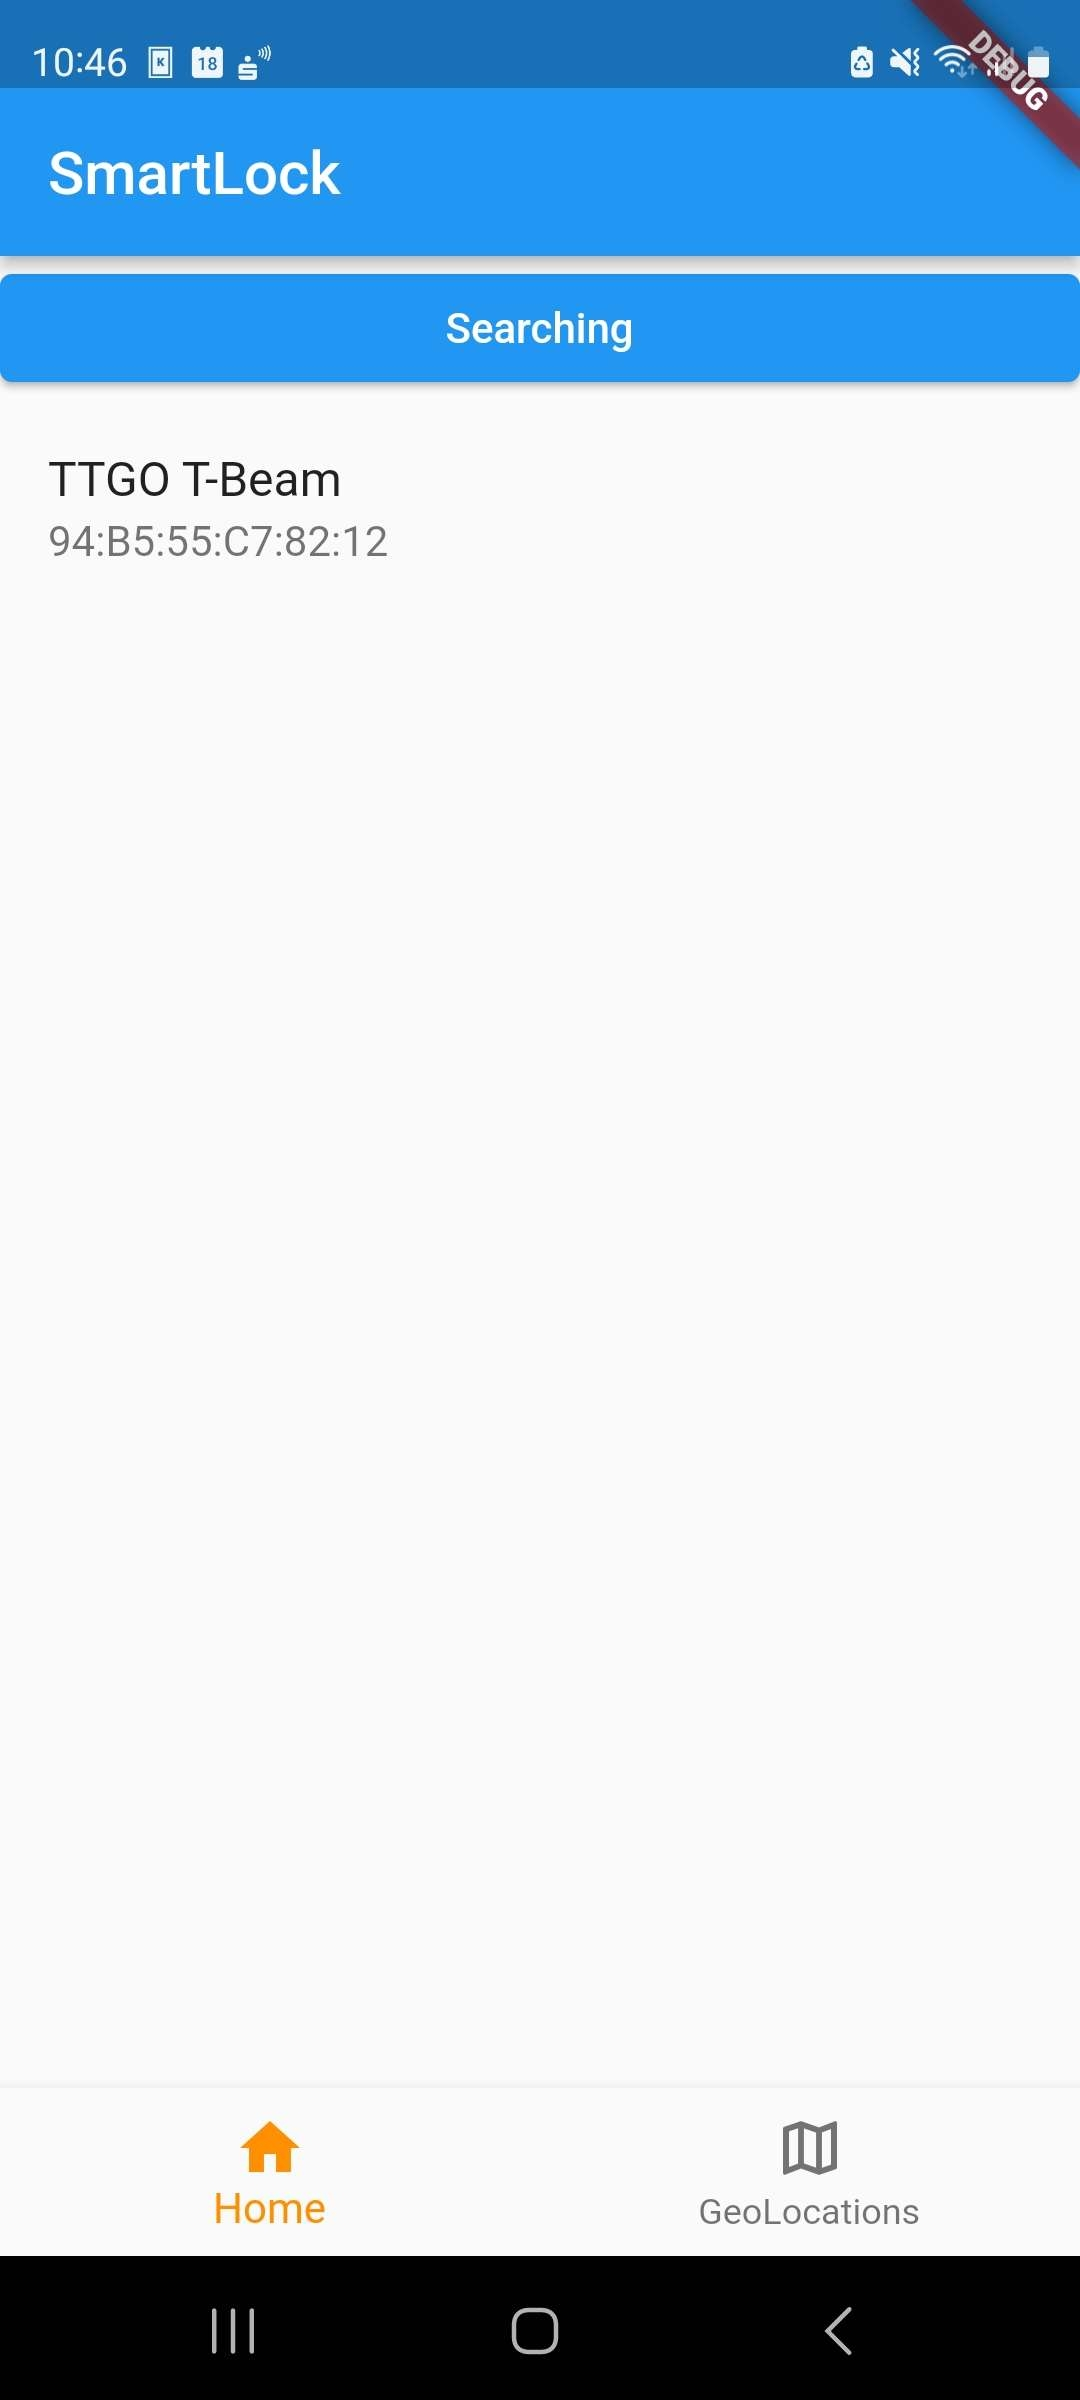
\includegraphics[width=0.3\textwidth]{images/search.jpg}
        \label{fig:search}
        }
    \hfill
    \subfloat[Verbundenes Schloss Öffnen und Schließen]{
        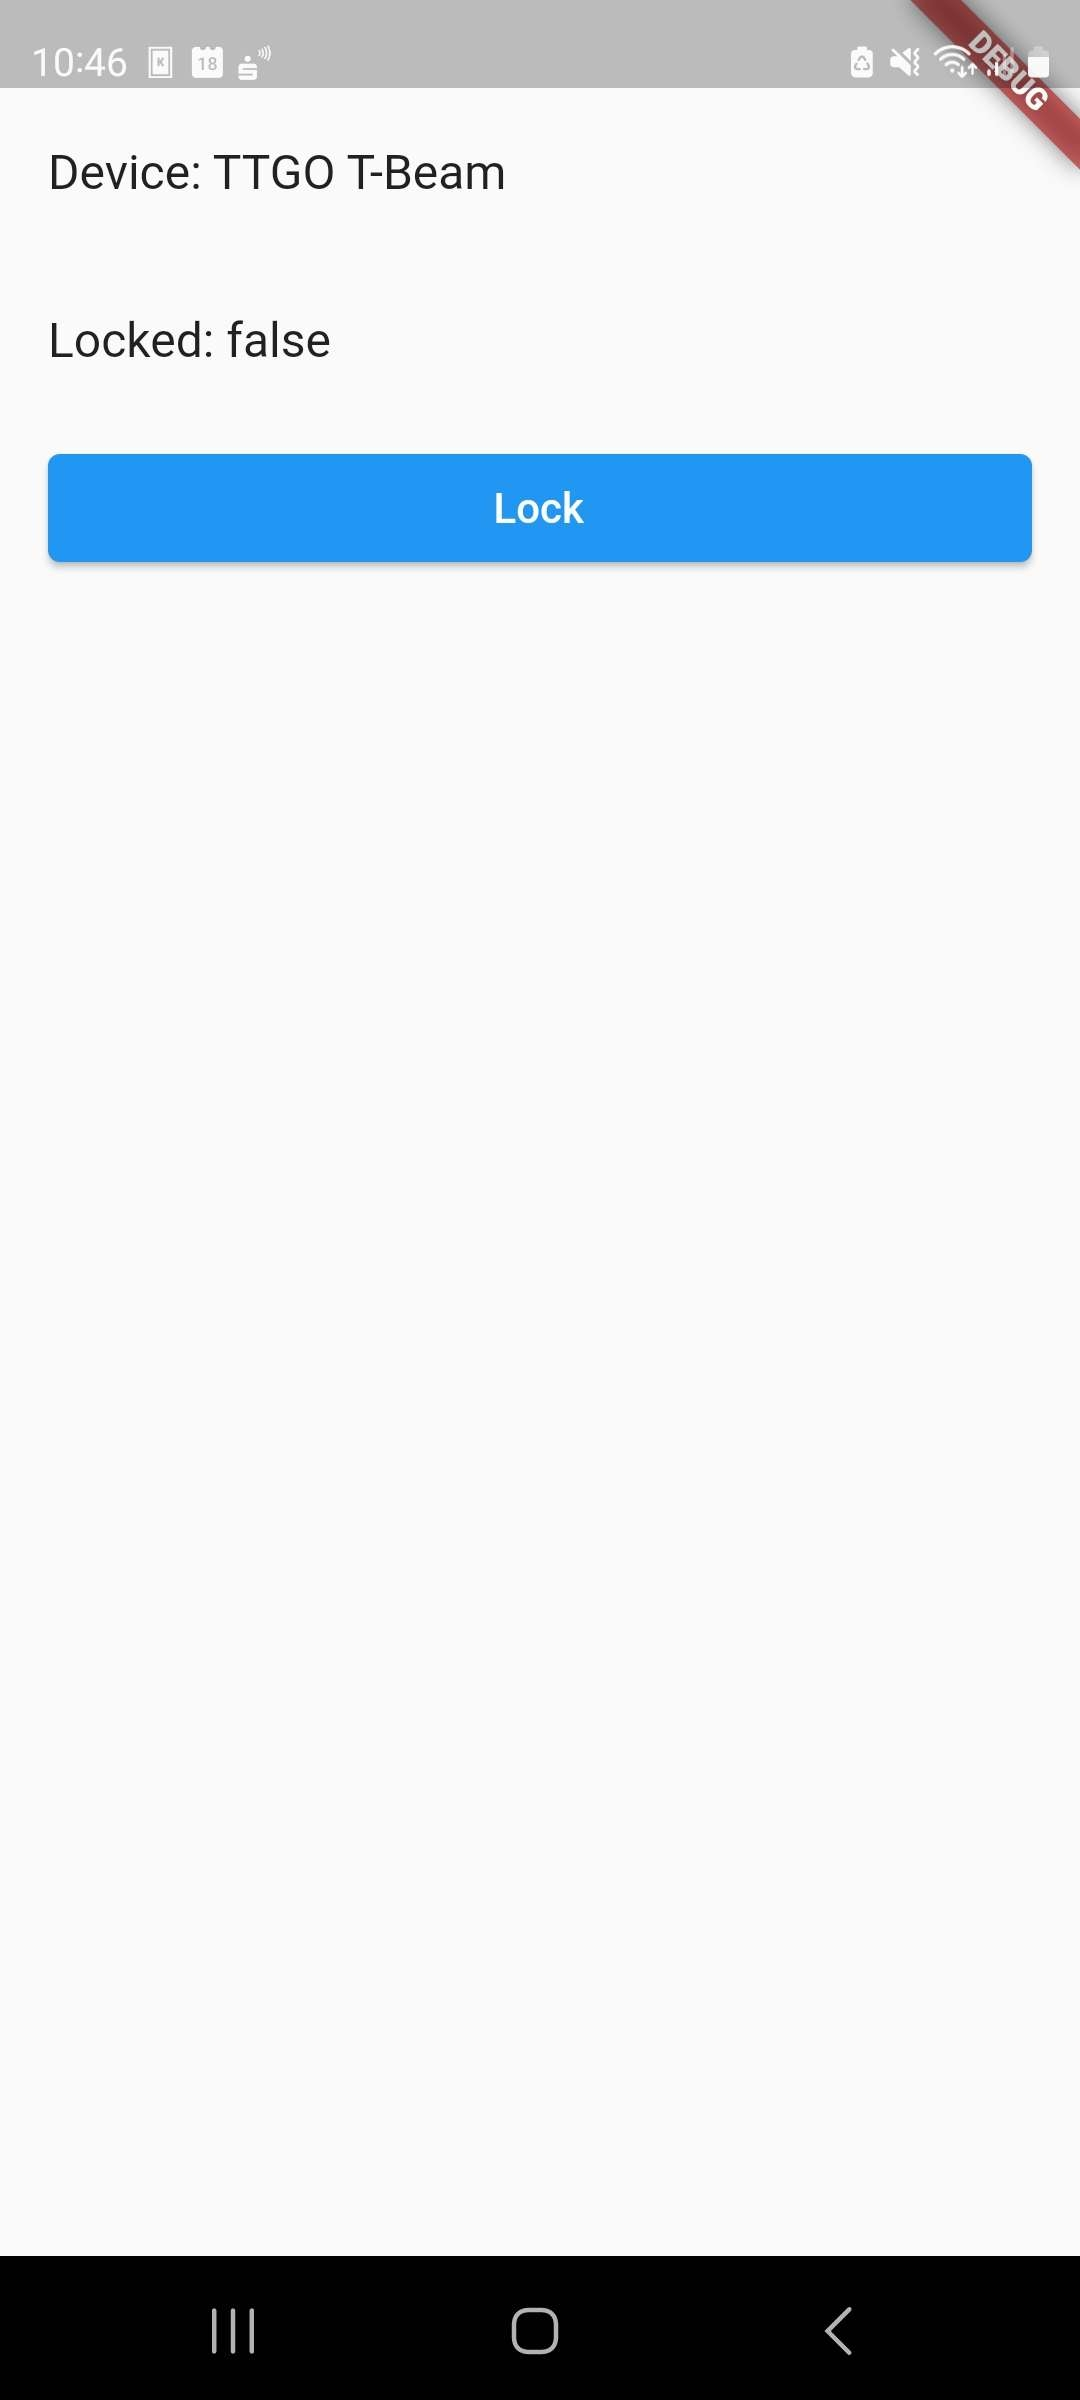
\includegraphics[width=0.3\textwidth]{images/connected.jpg}
        \label{fig:connected}
    }
    \caption{Smart Lock App: Aufbau}
\end{figure}